% Chapter 7

\chapter{Error Analysis and Quality Assurance} % Main chapter title

\section{Systematic Errors}
\subsection{Event Plane Resolution}
\begin{figure}[htbp]
  \centering
    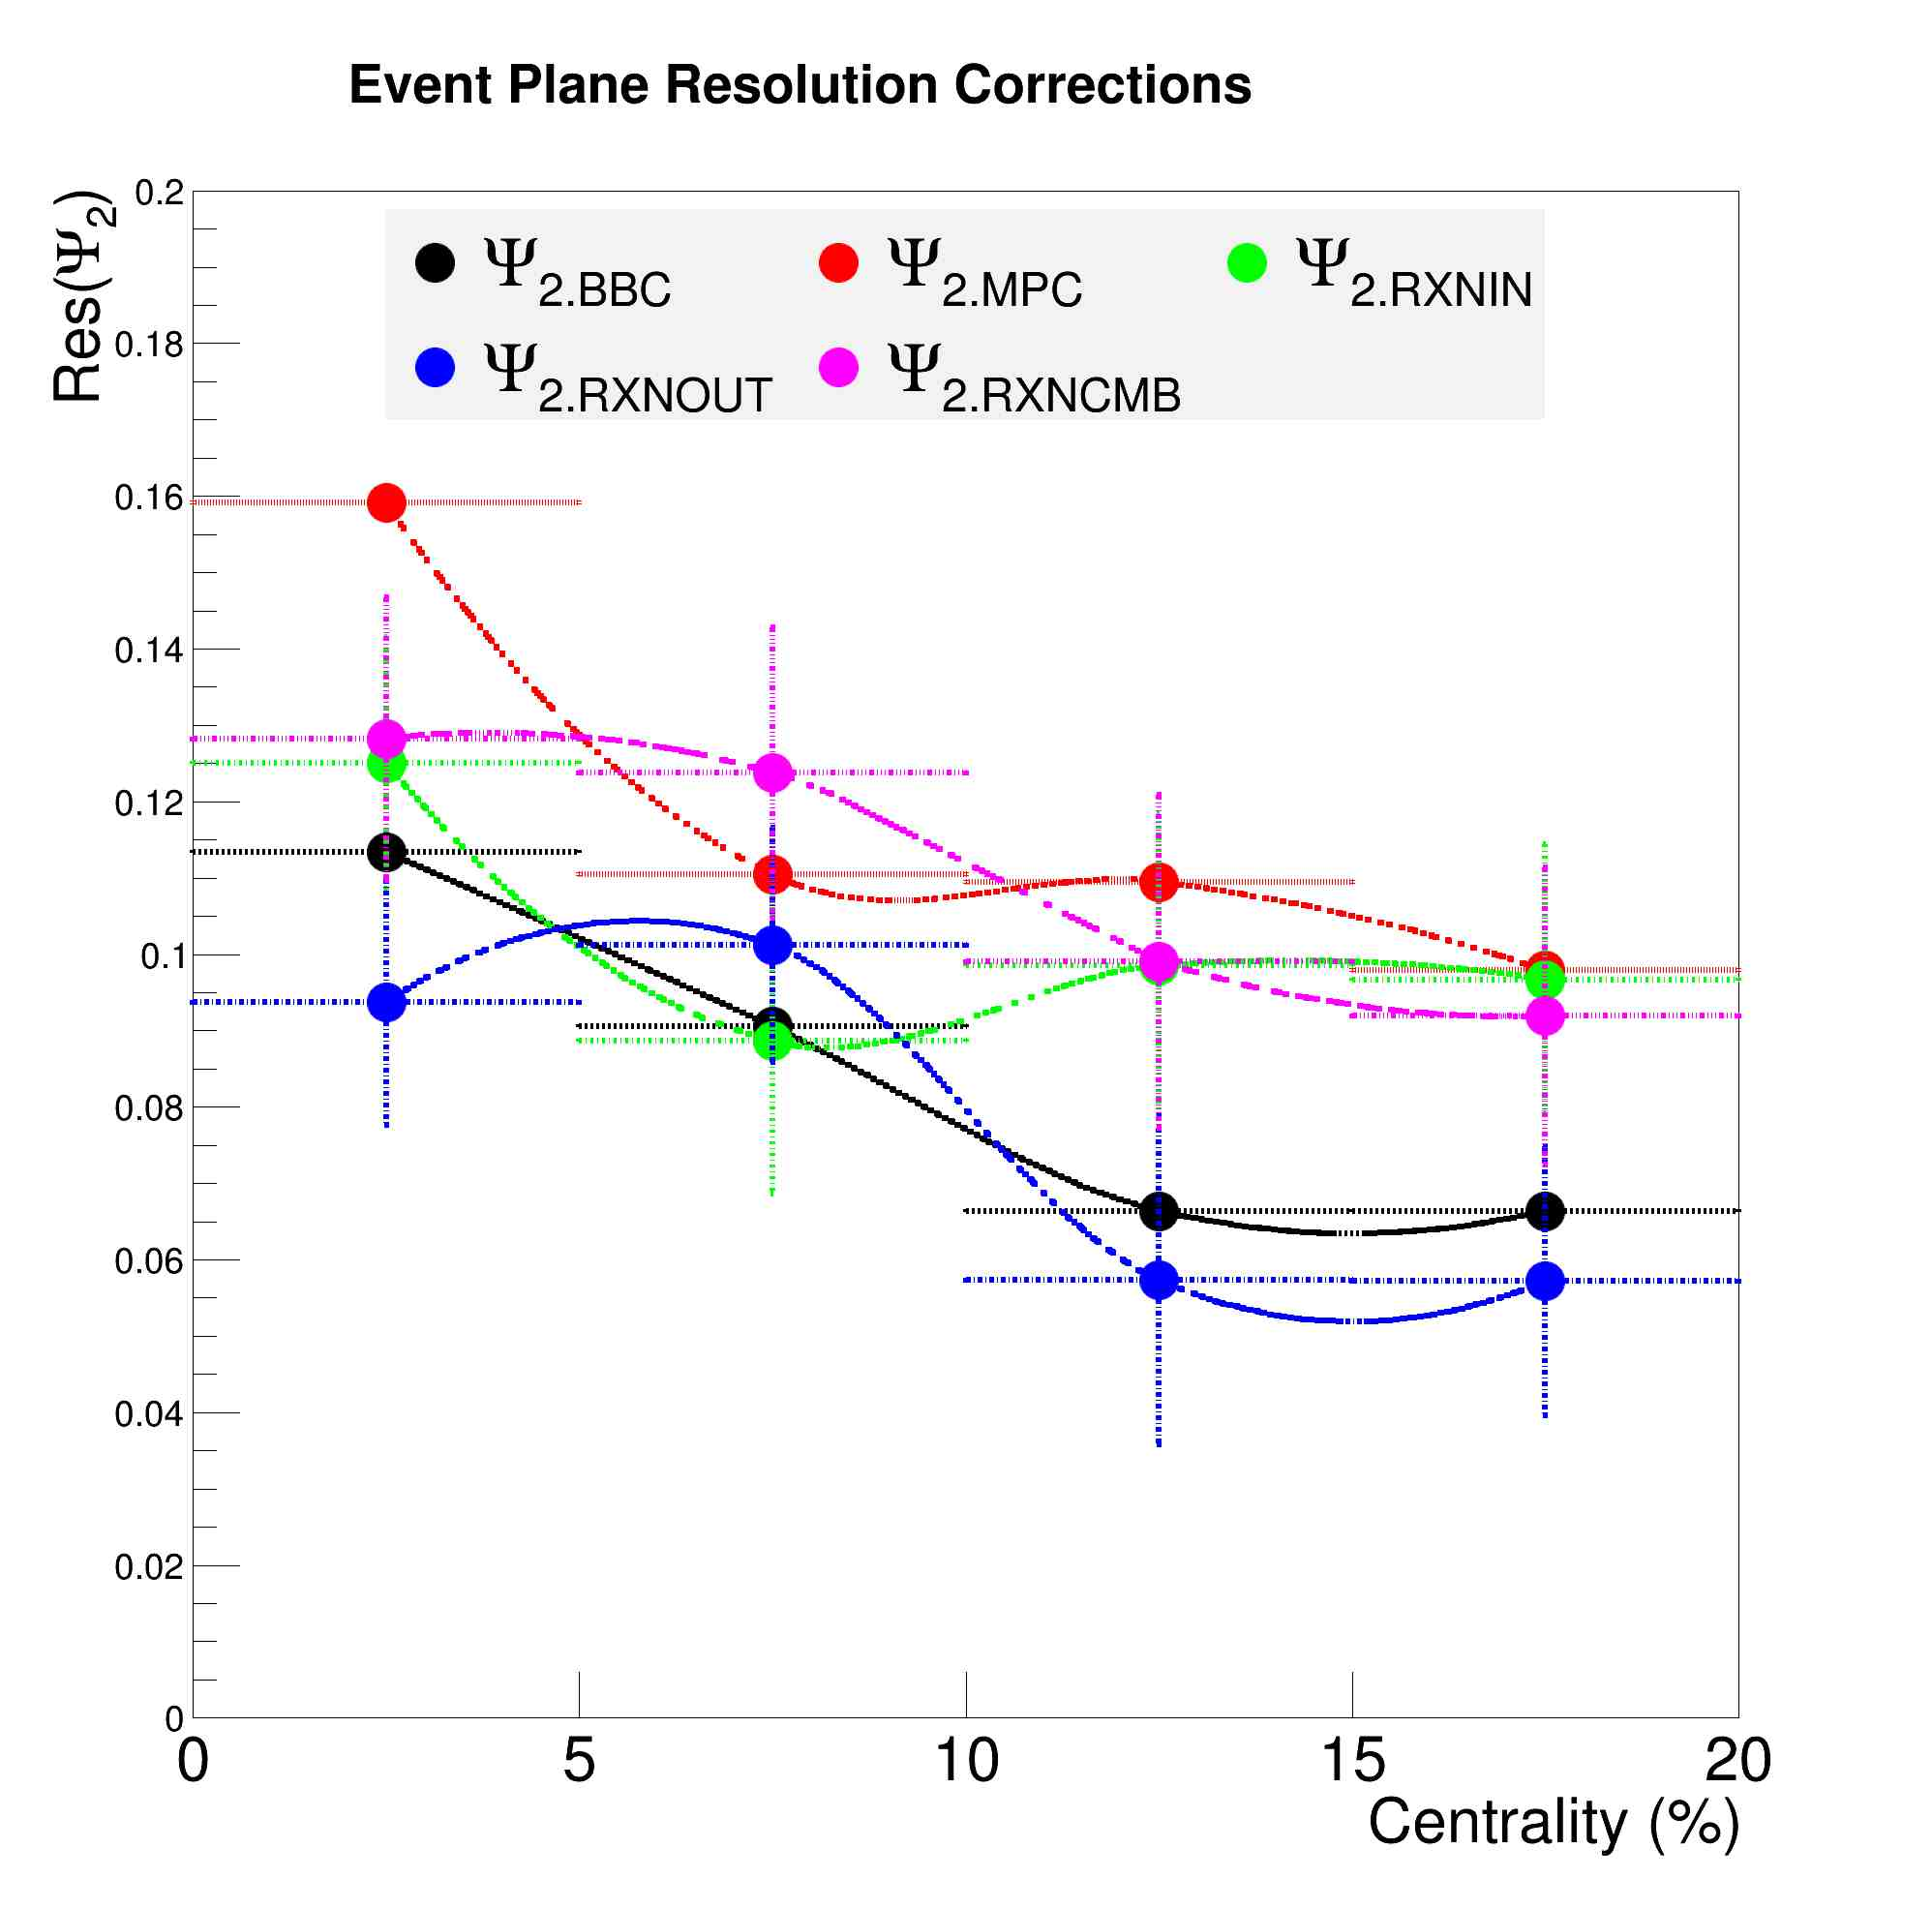
\includegraphics[width=0.7\textwidth]{evtQA/EPresr8da.jpg}
    \rule{35em}{0.5pt}
  \caption[Event Plane Resolution for BBC, MPC, and RXNP.]{Event Plane Resolution for BBC, MPC, and RXNP. Resolution calculation by Takao Sakaguchi\citep{pi0v2run8dau}. see also Table \ref{EPrestable} in Appendix \ref{app:data}}
  \label{fig:EPres}
\end{figure}
As mentioned in section \ref{sect:epres}, limitations of the detectors to precisely resolve the event plane contribute to a weaker anisotropic flow measurement. This is exacerbated by the asymmetric nature of the d+Au system. By RHIC convention and PHENIX construction, the north side is the ``deuteron-going'' side and the south side is the ``gold-going'' side. The significant increase in the number of nucleons in a gold nucleus result in more track multiplicity with which to determine the event plane. Because of this, event plane determination using south arm detectors is significantly easier and more accurate, as evident in fig \ref{fig:evtpln}. This combination of higher track multiplicity and flatter event plane distribution in the BBC make specifically the south BBC the best detector with which to determine the event plane. However, additional independent measurements of the event plane are still useful as they can be used to correct resolution limitations since three independent measurements of one event plane are necessary in order to use the Three Subevent Method. The Event Plane resolution corrections used in this analysis that are displayed on figure \ref{fig:EPres} were calculated for Run 8 d+Au by Takao Sakaguchi, et al. for a flow analysis of $\pi_0$ in the same system. Since the only value here I use for this analysis is the most central bin using the BBC, the uncertainty in the resolution here can be assigned a 1\% systematic uncertainty.

\subsection{Centrality Resolution}

\subsection{Particle Identification Methods}
There are three sources of error that can come from the identification of these particle species. Since the separation of signals is dependent on the time of flight and the momentum, uncertainty in either of these propagates to the error in identification. Furthermore, imperfections in the goodness of fit for the Gaussian models can systematically miscount particles contributing to further uncertainty in flow coefficients.

\subsubsection{Momentum Uncertainty}
Track momentum is determined by track curvature in the DC/PC1 as described in section \ref{trkrecosect}. Track curvature and certainty of this calculation is correlated to the ability to match hits in the DC and PC which is quantified by the \textit{track quality} designation. As mentioned, only tracks which have at least 3 hits in the DC and PC1 are accepted for analysis. Additionally, TOF and PC3 tracking adds additional confidence to the tracing of individual hits to reconstructed tracks. Track projections that pass the quality cut in the PC1 are projected onto the TOF and PC3 and only hits that fall within $3\sigma$ of the projected hit are accepted for analysis. Furthermore momentum reconstruction resolution has been studied with single particle simulations\citep{Mitchell:2002wu}. This resolution was shown to be linear in $p_T$ with the highest $p_T$ bin used in this analysis (5 GeV/c) having a resolution of 2\%.
 
\subsubsection{TOF Timing}
Since the TOF boasts a very high timing resolution and since the preamplifier gains, cable lengths, and various other systematics can affect the timing measurement from strip to strip, it is important to calibrate the response across all the strips in the TOF. Conventionally, the tracks are shifted to some expected value. Since pions are by far the most plentiful particles created in heavy ion collisions, we pick them to be our normalization. Specifically the track time distribution is plotted for each strip individually. We know the start of the event time as given by the BBC and we know the expected time of flight for a pion ($t_{\pi}$) of mass $m_{\pi}$ with a measured momentum, $p$:

\begin{equation}
t_{\pi} = \sqrt{\frac{m_{\pi}}{p^2} + \frac{1}{c^2}}.
\end{equation}

We then subtract this offset from our measured time to set the average track incidence time to around 0.

\begin{equation}
\Delta t = t_{TOF measured} - t_{collision} - t_{\pi} 
\end{equation}
 
\begin{figure}[htbp]
  \centering
    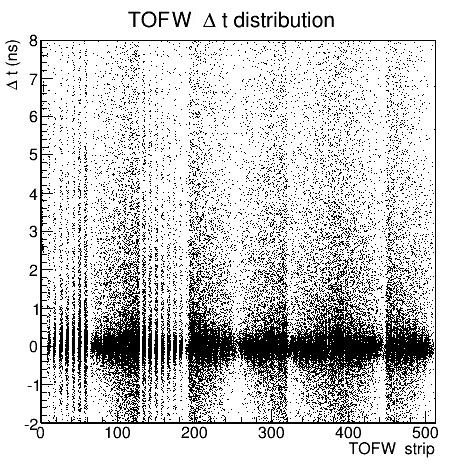
\includegraphics[width=0.5\textwidth]{evtQA/ttofwdist.JPG}
    \rule{35em}{0.5pt}
  \caption[Timing calibration in the TOF.W]{Timing calibration in the TOF.W, $\Delta$t vs TOF.W strip id}
  \label{fig:tofwdist}
\end{figure}

Furthermore, the TOF.W has a known resolution of $\sim 80 ps$. Propagating this error through eqn \ref{eqn:m2tof} with the known distance from the vertex of the TOF.W and a maximal value for this analysis of $p_T=5$ GeV/c, the maximum variance in $m^2$ due to timing capabilities is $\pm 4 \times 10^{-9}$ GeV/c which is negligible.

\subsubsection{Uncertainties from Gaussian Models}
Species purity is integrated out to $2\sigma$ which accounts for 95.45\% of particles about the mean of their distribution. Therefore systematics due to mixing in the tails of the particle distributions is at most 4.55\%. Gaussian distributions do not perfectly match the particle distributions, however it can be shown that and over and under counting done by the models is uniform across each bin in $d\phi$ for a given bin of $p_T$ and only serves to shift the y-position of the flow curve a net value up or down without changing the value of the harmonic for the range $p_T \leq 3$ GeV/c. For $p_T \geq 3$ GeV/c greater systematics are evident as the widths and means of the particle distributions change. 

\subsection{Detector Acceptance}




\pagebreak
\pagebreak
